\chapter{Result Analysis}
\section{Robot Movement}
The robot movement in various directions was performed by pressing the a, w, s,
d keys on the keyboard. The robot reacted spontaneously. This was accomplished
with the help of Wi-Fi and a delay less TCP-IP socket transfer protocol.All the functionality of 
the TCP-IP socket protocol were successfully implemented without any errors. Upon pressing of the keys the
respective robot movements in different directions were observed.
\begin{figure}[h]
\centering
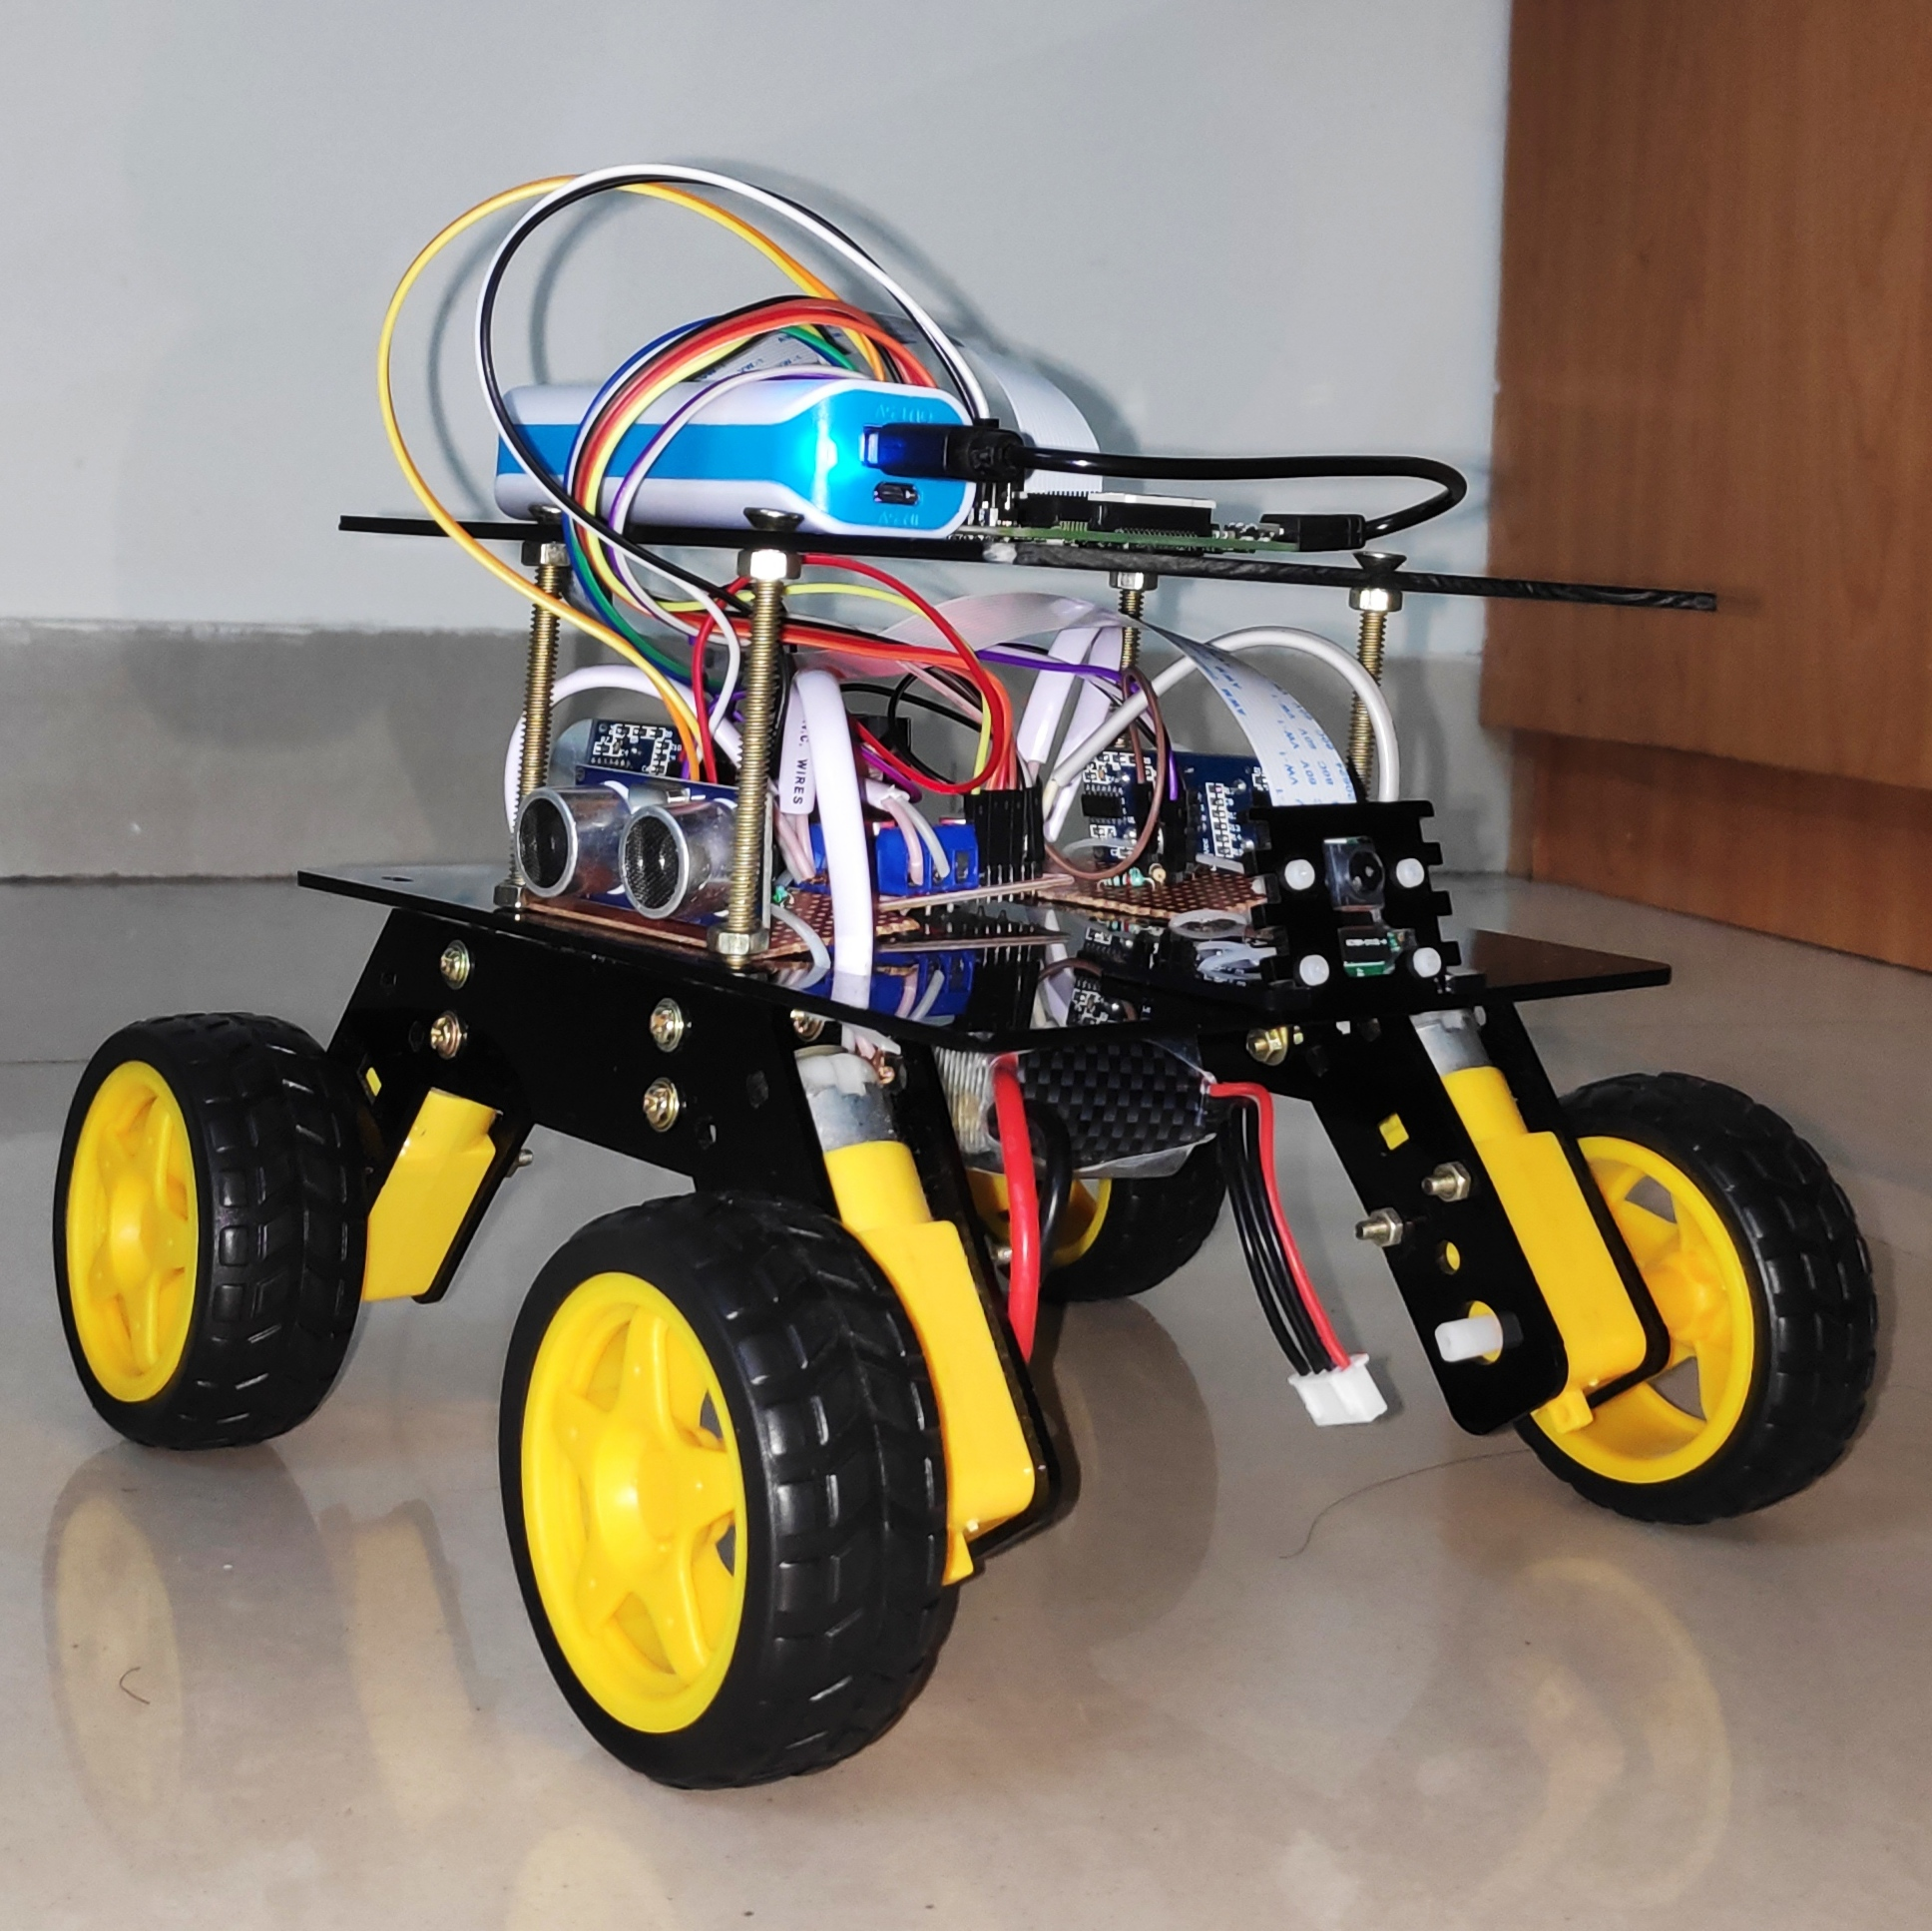
\includegraphics[scale=0.09]{robo3.jpg}
\caption{Complete Robot Setup}
\end{figure}
\section{Video Streaming}
We also successfully captured video frames using a Raspberry Pi Camera and displayed it on a flask website.
\begin{figure}[h]
\centering
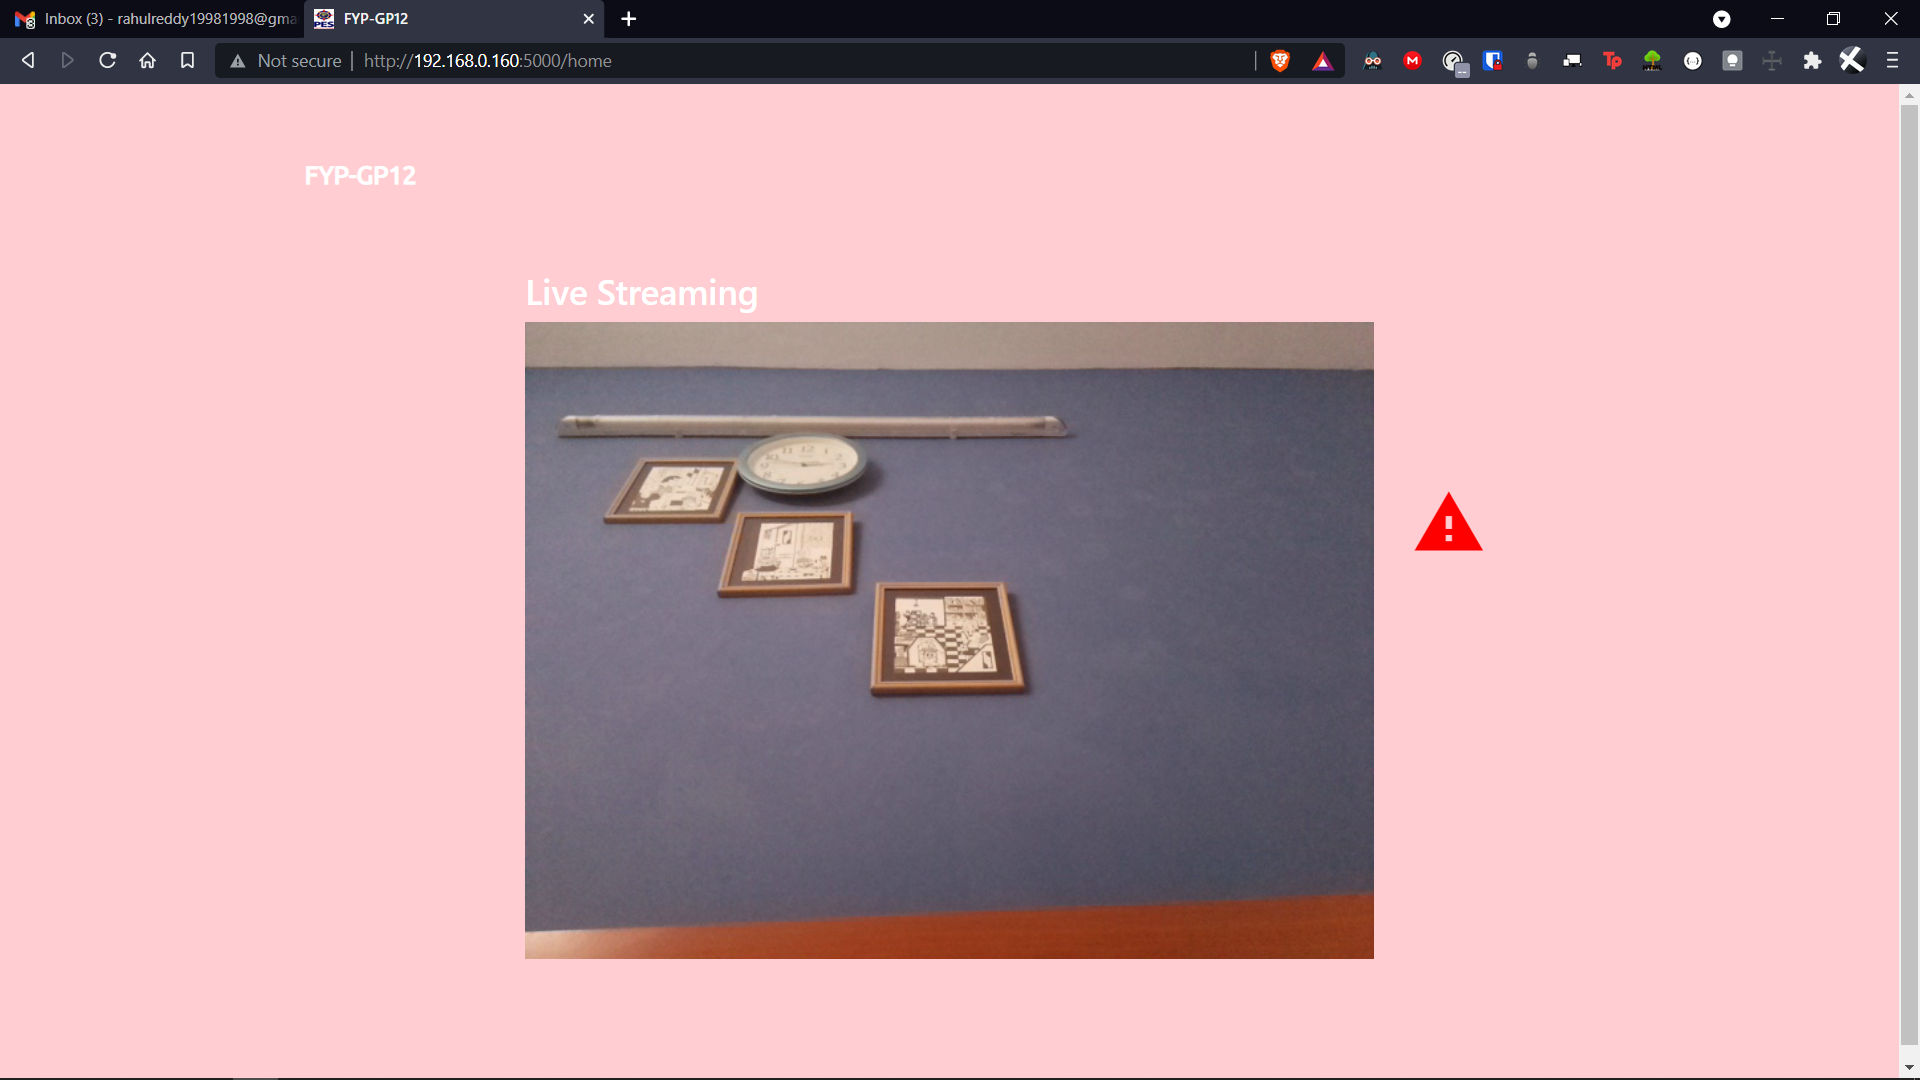
\includegraphics[scale=0.15]{video.png}
\caption{Video Streaming Webpage (Screenshot)}
\end{figure}
\section{Sensor Data Acquisition}
We also hosted an API which helps in the acquisition of Ultrasonic sensor data. We then 
request sensor data from this API to provide alerts for the left, right and rear ends 
of the robot on the web-page. The API worked according to the intended functionality.The Video Stream and the API together helped us in remotely controlling the robot.
\begin{figure}[h]
\centering
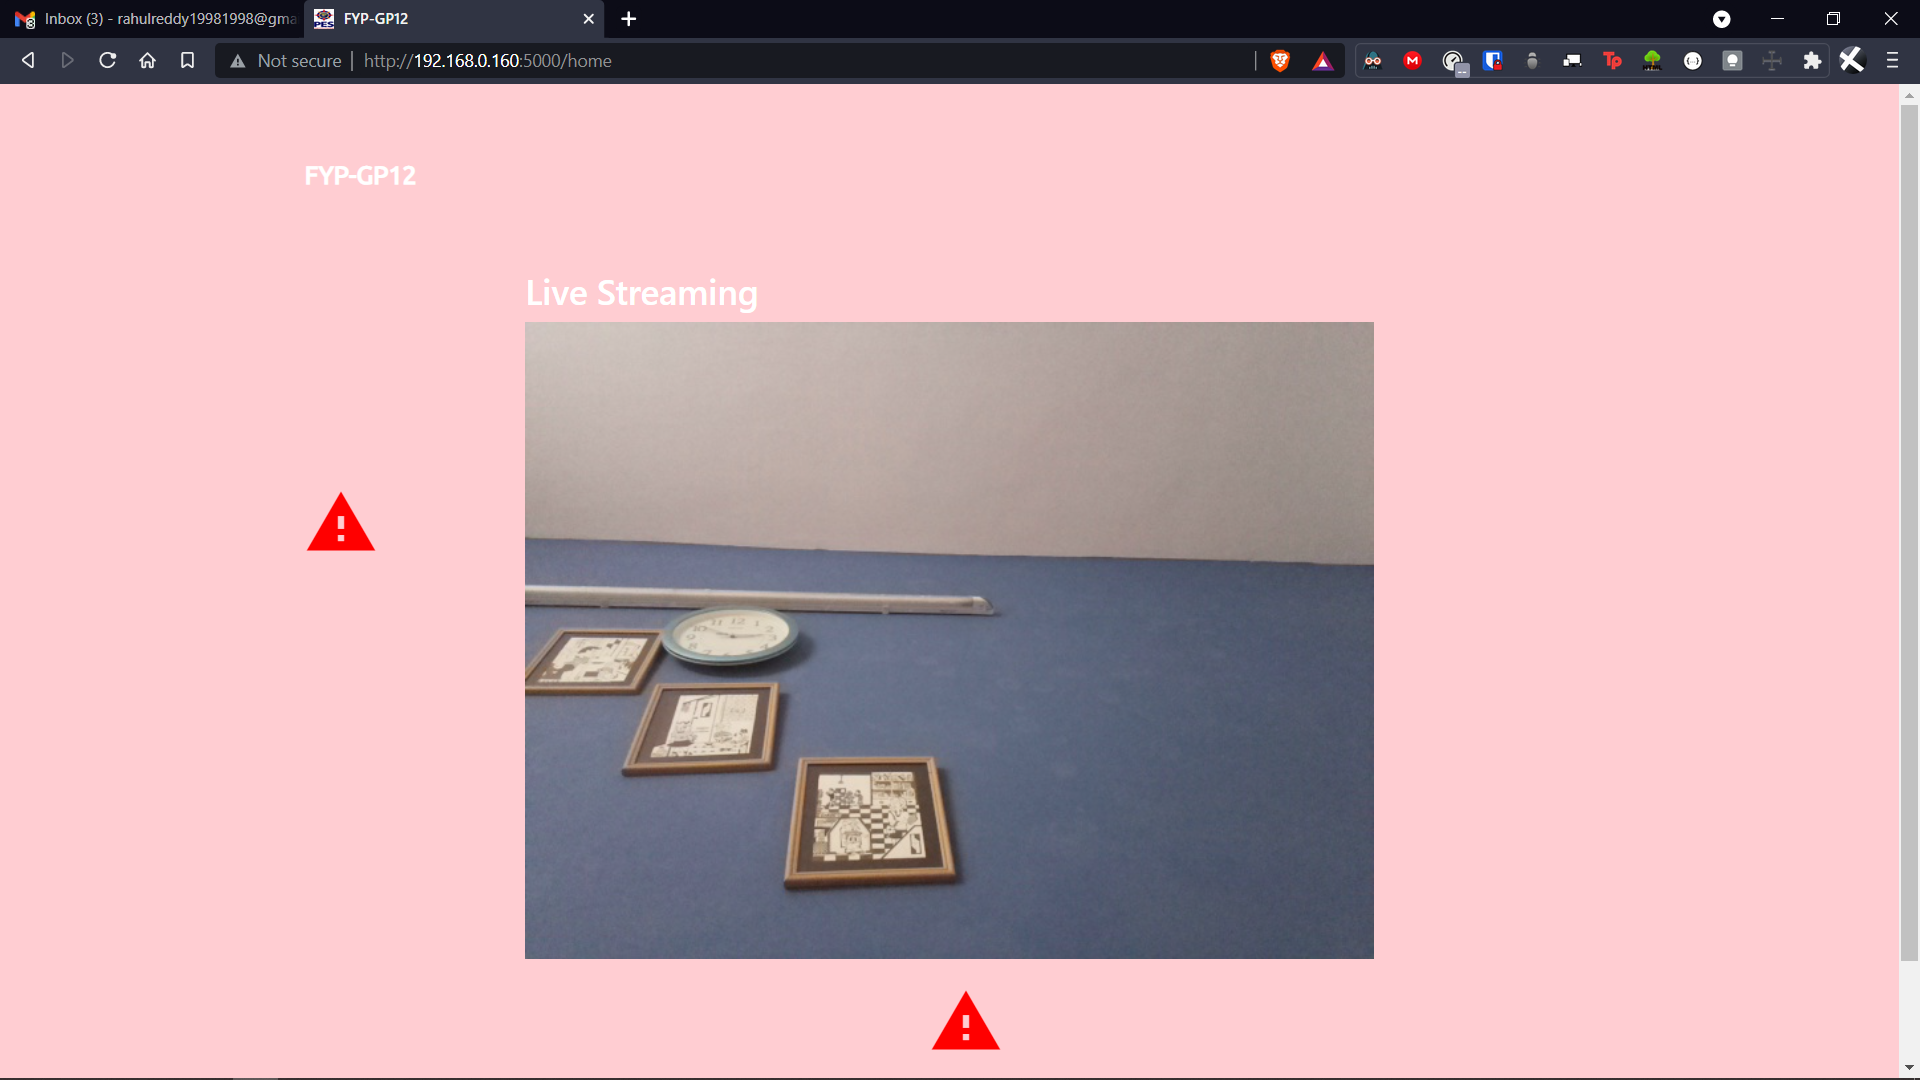
\includegraphics[scale=0.15]{sensorshow.png}
\caption{Obstacle detected in Left and Rear Sensors}
\end{figure}
\section{Solar Charging}
In addition we also built a solar charging circuit in-order to charge the batteries. This made our project more environment friendly and helped conserve Non-Renewable Energy resources.